\section{Què és?}
El \emph{software} o \emph{programari} és el conjunt dels programes informàtics, procediments i documentació que fan alguna tasca en un ordinador. Per tant, qualsevol eina que s'executa en el nostre ordinador, que té una tasca definida, es pot definir com a programari. Casualment, la major part d'eines que executem diàriament en els nostres ordinadors, duen a terme alguna tasca
(navegar internet, crear un document, consultar el correu electrònic, etc). Per tant, un ordinador sense programari, serveix de ben poc.

\emph{Paint}, \emph{Photoshop}, \emph{GIMP}, \emph{Steam}, \emph{Firefox}, \emph{Dropbox}, \emph{Office}, \emph{Avast}... tots aquests noms fan referència a programes, software. És 
sense dubte complicat imaginar un ordinador sense cap d'aquests elements instal·lats, veritat?

\section{Com es crea?}
El programari, encara que sembli redundant, es programa. Els \emph{programadors}
són enginyers que desenvolupen aquest programari. Per a crear software, s'utilitzen
\emph{llenguatges de programació}, que n'hi han molts (\emph{C, Python, Lisp, Haskell...})
i cadascun amb el seu propòsit diferent. Quan s'ha completat el disseny d'un programa
(es a dir, s'ha programat el \emph{codi font} \footnote{Instruccións que se li donen al
llenguatge de programació}), aquest es \emph{compila} a \emph{codi de màquina} \footnote{Text indesxifrable per al cervell humà, però que els sistemes operatius entenen}, que l'ordinador llegeix i executa.

Si es detecta un mal funcionament en algun moment en l'execució del programa, anomenat \emph{bug}, els
programadors revisen el codi font, fan les correccions necessàries, compilen el programa,
i el distribueixen altre cop.

Quan l'usuari adquireix el programari en format de codi de màquina, o \emph{binari}, només el pot
executar. És molt complicat desxifrar el codi original a partir del producte final, però és una
pràctica que solen realitzar les comunitats de \emph{crackers}, i s'anomena \emph{enginyeria inversa}.

Però no només els desenvolupadors de programari són qui compilen el codi font; depenent de la forma
de distribució del software, l'usuari final pot compilar el software, i fins i tot, fer-hi modificacions. Però, que l'usuari tingui aquesta oportunitat o no,  dependrà de si el software que ha adquirit es regeix per una llicència \emph{lliure} o \emph{propietària}.

\begin{figure}[ht!]
\centering
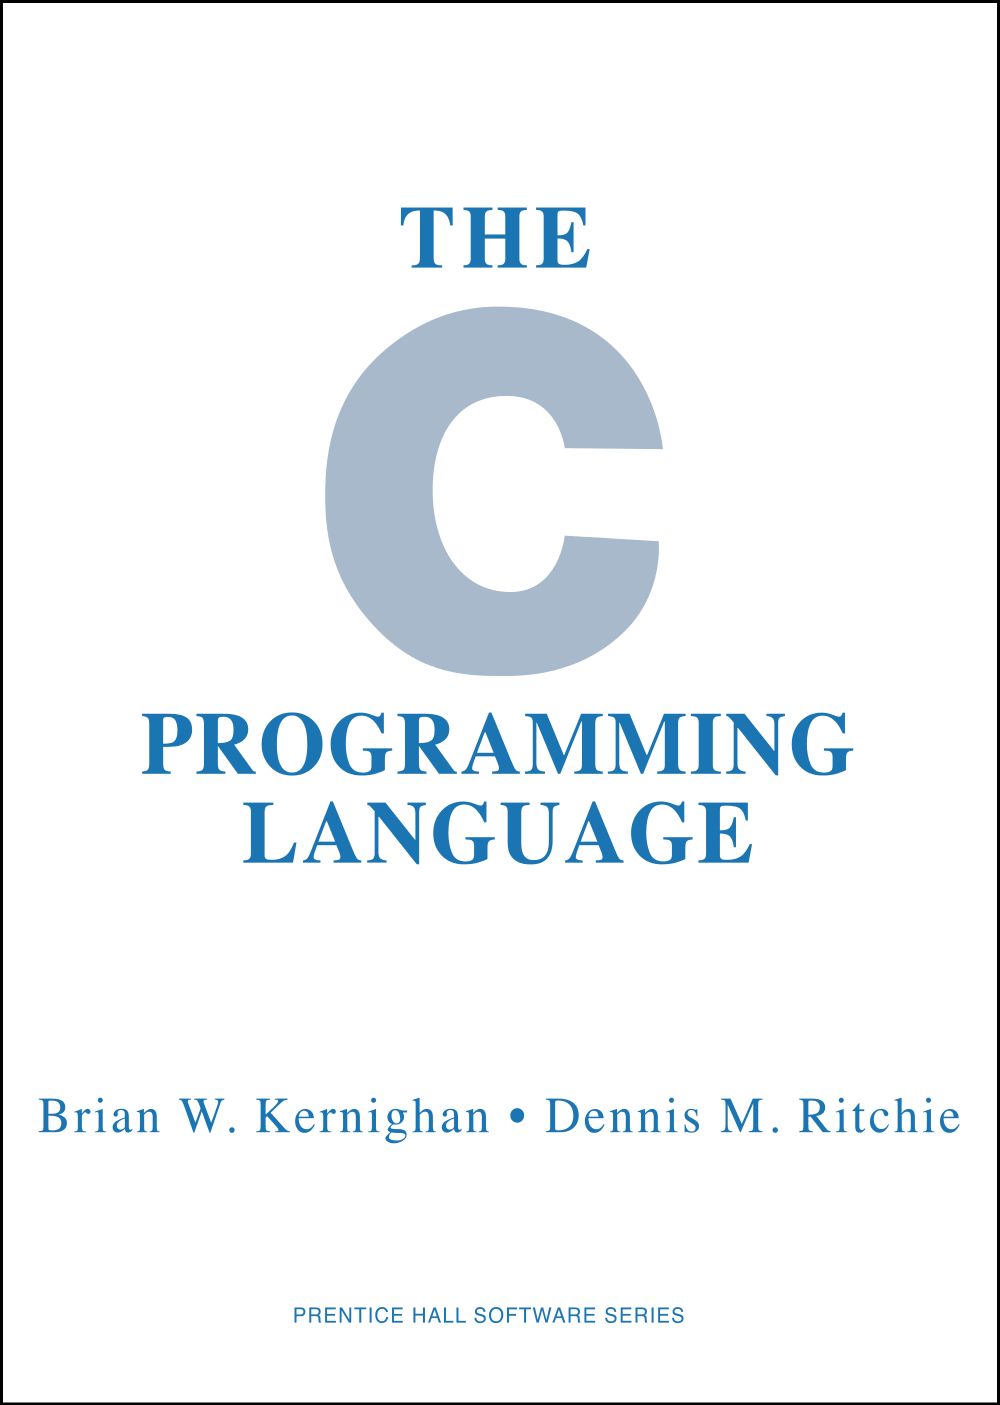
\includegraphics[height=75mm]{data/clang.png}
\caption{Portada del llegendari llibre que explica programació amb el llenguatge \emph{C}, de \emph{Kernighan} i \emph{Ritchie}, els dos desenvolupadors principals.}
\label{websshare}
\end{figure}
